\chapter{Extending 2D DGGS's to Three Dimensions} \label{chap:extension}
While SDOG and its variants proposed in the previous chapter have many desirable properties, it may not be the ideal 3D DGGS in all circumstances.
The varying uses for a DGGS means each application has different needs of the DGGS it employs.
As such, no single DGGG---2D or 3D---is ideal for every use case.
Therefore, there is a need for many different DGGS's, each with unique properties and intended use cases.


Addressing the needs of different applications, researchers have developed a large variety of different 2D DGGS currently available; the creation of new 3D DGGS's should build off these existing methods.
A natural way to do so is with a method to extend a DGGS to 3D, as seen in~\cite{xie2013interactive} and~\cite{sirdeshmukh2019utilizing}.
However, existing extension methods are not generalizable to any possible DGGS and fail to address cell degeneration toward the centre of the grid.
In this chapter, we aim to address these shortcomings.
We present a general method for extending \textit{any} existing DGGS, referred to as the input DGGS, to the third dimension using a semiregular degenerate refinement strategy.
This extension is done with care to allow the efficient and straightforward transference of data between 2D and 3D while preserving---as best as possible---desirable properties of the input DGGS in the 3D one.
Figure~\ref{fig:extension} shows an overview of the method.
This chapter discusses only the creation of grid geometry; mapping and coding are discussed in Chapters~\ref{chap:mapping} and \ref{chap:coding}, respectively.


\begin{figure}[ht!]
	\centering
	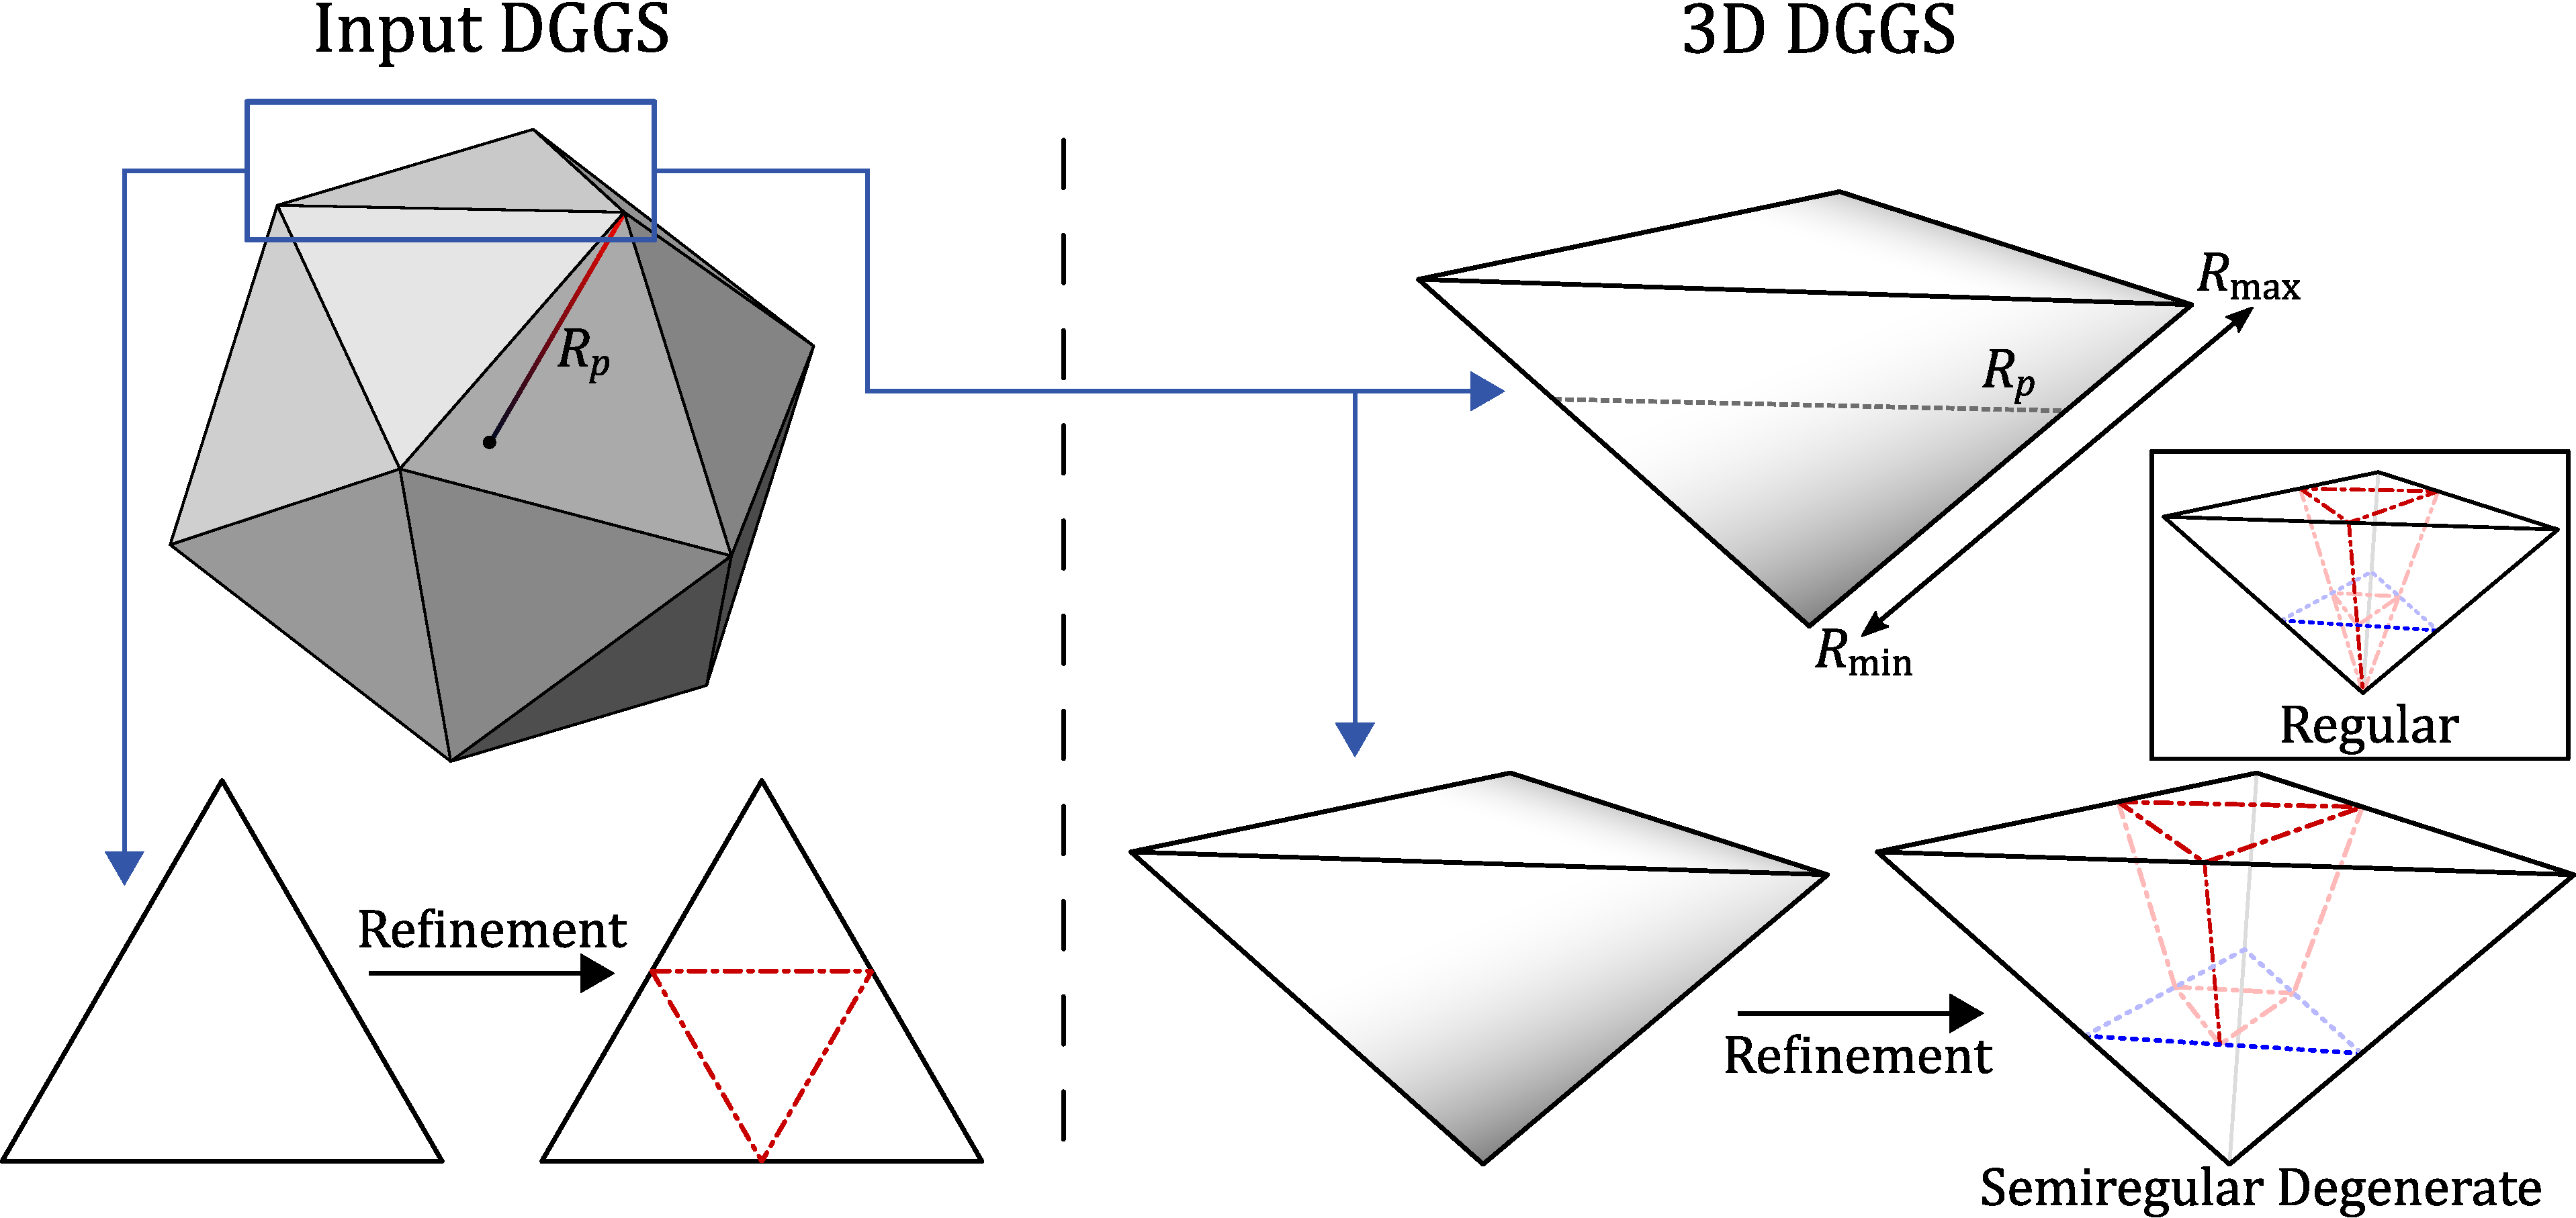
\includegraphics[width=\textwidth]{grid-extension-overview.pdf}
	\caption[Overview of the grid extension method]{
		Overview of how the input DGGS is used to define the geometry of the 3D DGGS.
		The faces of the initial polyhedron of the input DGGS are first extruded to create the prismatoid base cells of the 3D DGGS.
		For refinement, the bases of these prismatoid cells are refined using the same refinement scheme as the input DGGS and combined with a radial refinement.
		A semiregular degenerate refinement is suggested; however, regular refinement is also possible
	}
	\label{fig:extension}
\end{figure}


The content of this chapter is taken from the article "General Method for Extending Discrete Global Grid Systems to Three Dimensions," authored by Benjamin Ulmer, John Hall, and Faramarz Samavati, which appeared in the journal \textit{ISPRS International Journal of Geo-Information} in a special issue on Global Grid Systems~\cite{ulmer2020general}.
Slight modifications have been made to maintain consistent terminology with the rest of the thesis.


\section{Prismatoid Grid Generation and Refinement} \label{chap:5:grid}
Using the input DGGS as a specification, our goal is to define the key elements of the corresponding 3D DGGS logically and consistently.
Below, we discuss the approach for generating the initial discretization and define regular and semiregular degenerate refinement methods. 


\subsection{Initial 3D Discretization} \label{chap:5:discretization}
Let $R_\mathrm{min}$ and $R_\mathrm{max}$ be the minimum and maximum radii that are to be supported by the 3D DGGS, respectively.
The initial 3D discretization, then, is generated from two copies of the initial discretization of the input DGGS at these radii with their edges connected.
For an input DGGS defined directly on the sphere, the radius is well defined.
For a polyhedron-based DGGS, we need to define this radius.
Since the polyhedron is serving as an approximation of the sphere, we define the radius of a polyhedron to be the radius of its circumscribed sphere.
Thus, all points on a polyhedron have the same `radius' (Figure~\ref{fig:layers}).


\begin{figure}[ht!]
	\centering
	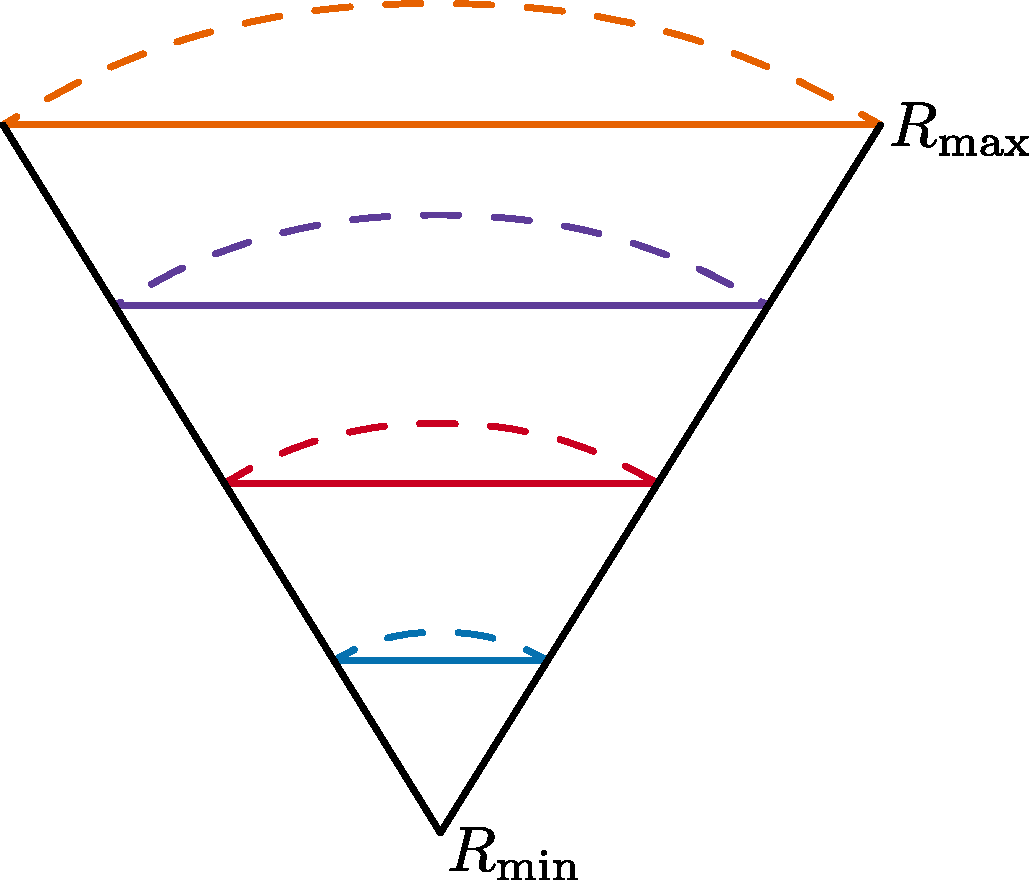
\includegraphics[width=0.5\columnwidth]{layers.pdf}
	\caption[How the radius of a polyhedron is defined]{
		We define the radius of a polyhedron as the radius of its circumscribing sphere.
		In this figure, all points on a solid line of a given colour have the same radius as they all have the same circumscribing sphere (i.e. lie on the same polyhedron).
		The corresponding spheres are shown in the same colours but with a dashed line
	}
	\label{fig:layers}
\end{figure}


If the minimum radius of the 3D DGGS is zero, the base cells are pyramids; otherwise, they are frusta.
In both cases, the cells belong to a parent class of polyhedra known as prismatoids.
For the remainder of this thesis, we assume that $R_\mathrm{min} = 0$; however, other values can be supported by truncating the resulting grid below the desired minimum.
With this discretization, each cell represents the full radial domain of the grid---subsequent refinements will address this issue.


\subsection{Regular Prismatoid Refinement} \label{chap:5:regular}
With an initial 3D discretization for the space of the grid system, we now need a method for refining cells to create more fine discretizations.
We also want to ensure that the 3D DGGS will make use of the same refinement scheme used by the input DGGS, referred to as the surface refinement.
For simplicity, we initially assume the surface refinement factor is 1:4; a generalization to other refinement factors is given later in Chapter~\ref{chap:5:factors}.


\begin{figure}[ht!]
	\centering
	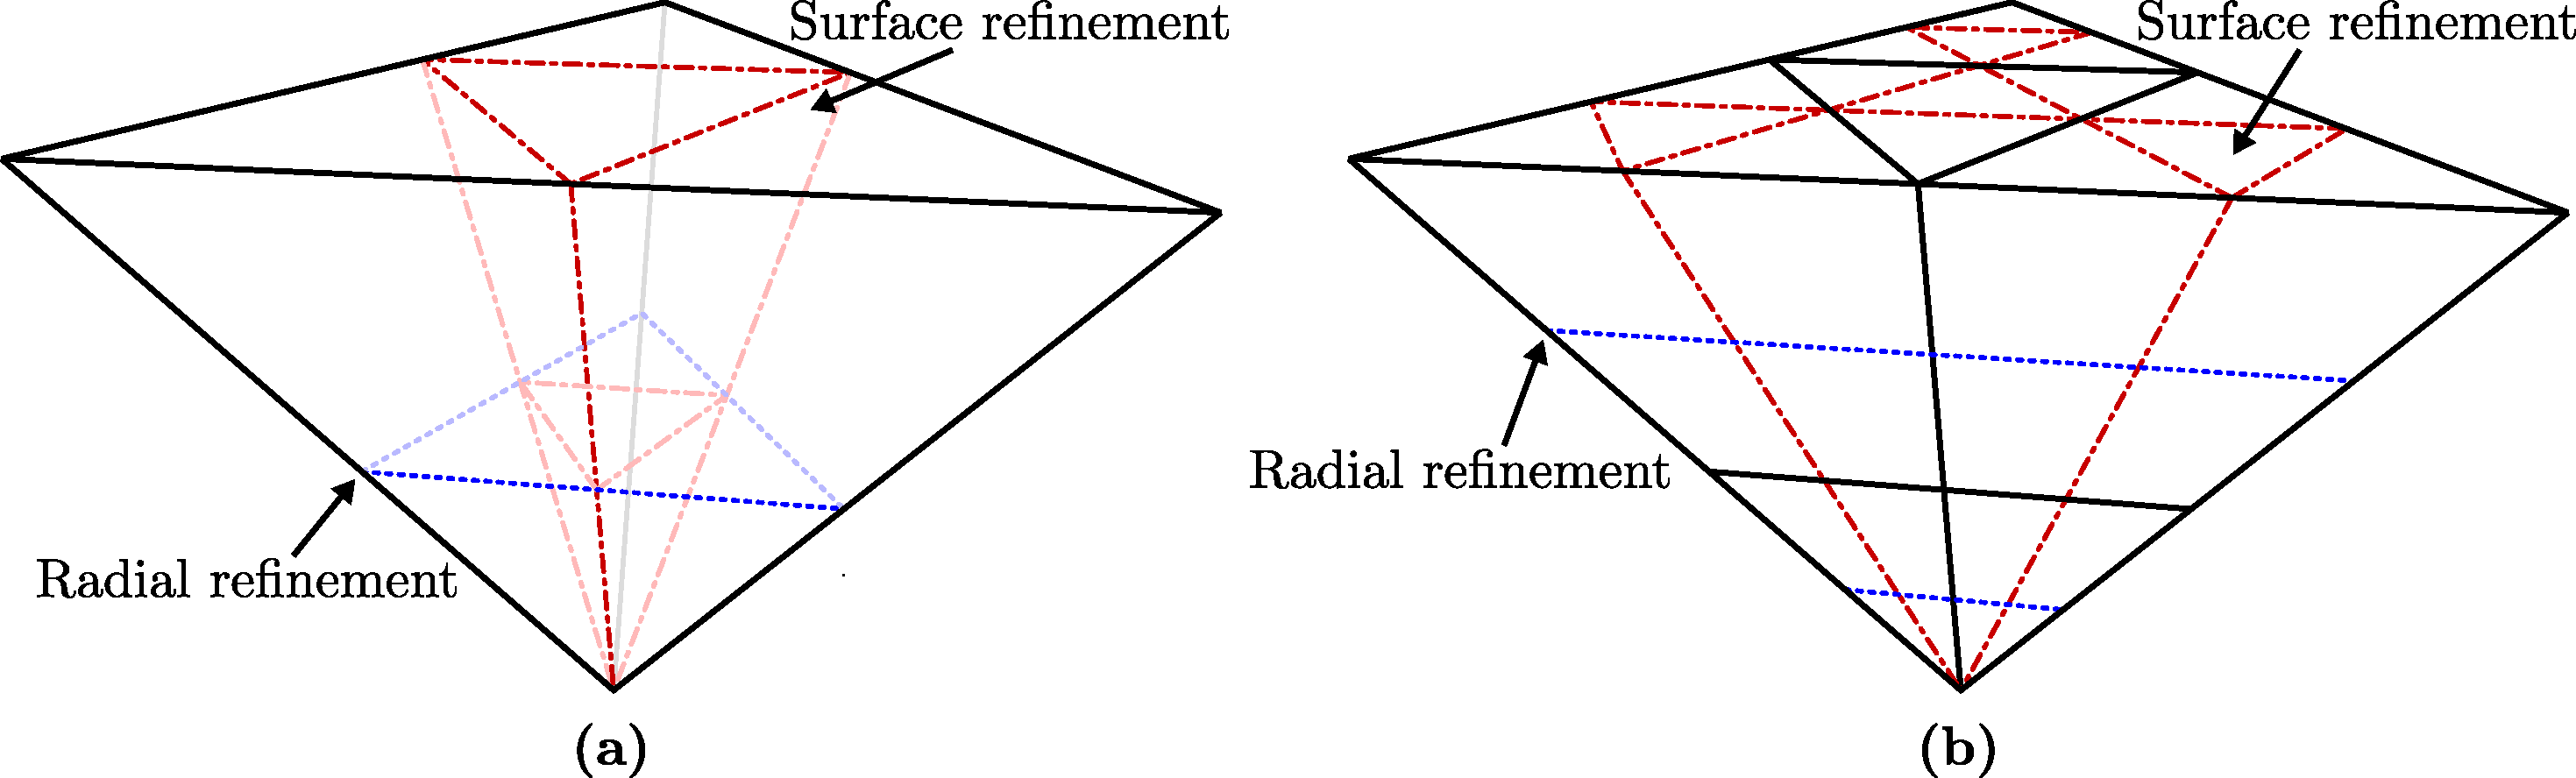
\includegraphics[width=\columnwidth]{reg-refinement.pdf}
	\caption[Regular prismatoid refinement]{
		Regular prismatoid refinement as applied to a single pyramid cell (a) once and (b) twice
	}
	\label{fig:regular}
\end{figure}


Figure~\ref{fig:regular} demonstrates the regular method for refining prismatoid cells.
The bases of the cells are refined using the surface refinement and the resulting edges extruded to meet.
At the same time, a radial split is placed at the midpoint of the two bases.
This refinement results in an inner and outer layer of cells, each containing the same number of cells as one another.
The outer layer is always composed of frustum cells, whereas the inner layer has the same shape as the cells that were being refined.
Defining the refinement in terms of layers of cells as opposed to individual cells allows for native accommodation of non-congruent surface refinements.


\subsection{Semiregular Degenerate Prismatoid Refinement} \label{chap:5:semireg}
While the regular prismatoid refinement proposed above is simple, it has the same issues near the central singularity as other Earth-centric 3D DGGS's.
To address this issue, we define a semiregular degenerate refinement for the prismatoid cells.
Aiding in this, we classify the layers of the grid as either central or normal.
We use $r_\mathrm{min}$ and $r_\mathrm{max}$ to refer to the minimum and maximum radius of a layer, respectively.
As with the polyhedra used for the initial discretization, these radii are equal to the radii of the circumscribing spheres.
Central layers are those that border the central singularity of the grid ($r_\mathrm{min} = 0$), and all other layers are considered normal.
By definition, at any resolution of the 3D DGGS, there is only one central layer.
Furthermore, the initial discretization is entirely composed of this central layer.
We continue our assumption of a 1:4 surface refinement factor from before.


\begin{figure}[ht!]
	\centering
	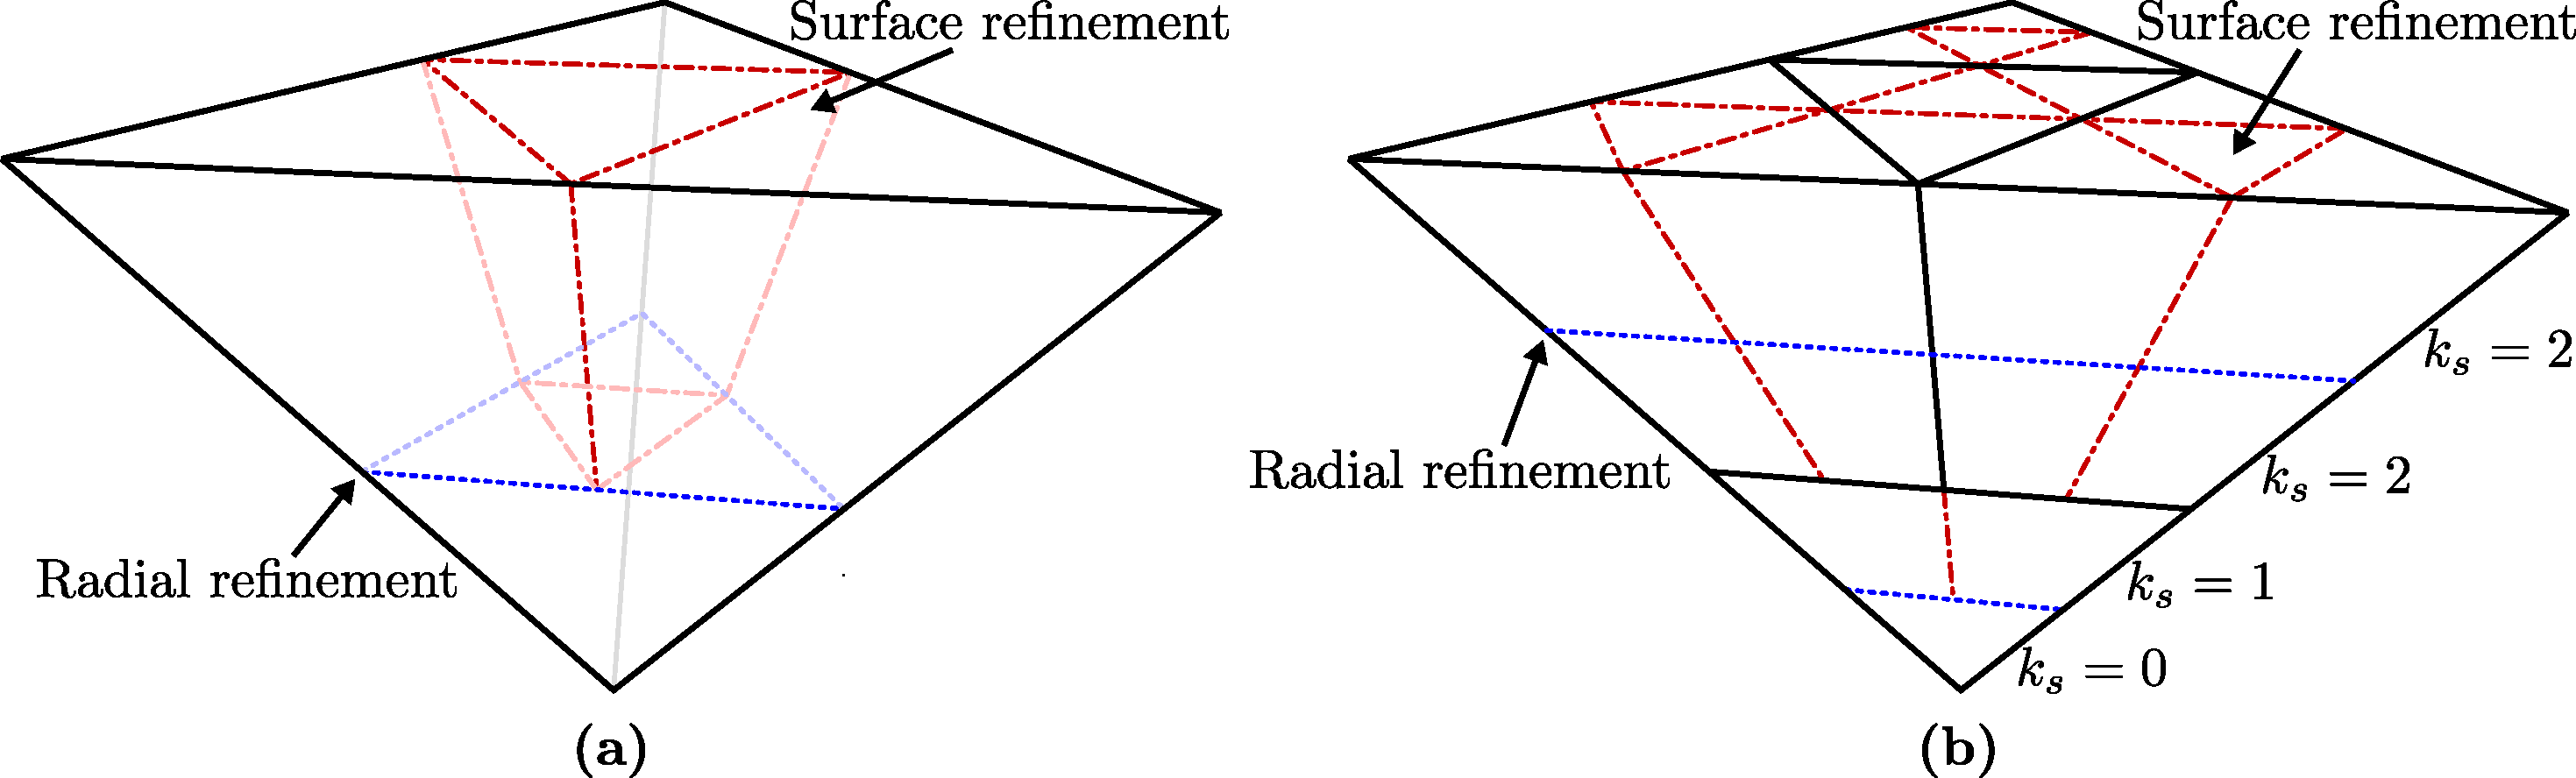
\includegraphics[width=\columnwidth]{semireg-refinement.pdf}
	\caption[Semiregular degenerate prismatoid refinement]{
		Semiregular degenerate prismatoid refinement as applied to a single pyramid cell (a) once and (b) twice.
		In (b), the number of times the surface refinement has been applied ($k_s$) is shown for each layer; see how the radial refinements of central layers separate regions of the grid with different values of $k_s$}
	\label{fig:semiregular}
\end{figure}


Just as with regular refinement, the bases of the pyramid cells are refined using the surface scheme with a radial split made in the middle of the layer.
However, to make this refinement semiregular degenerate, the new edges do not extend beyond the radial split in the direction toward the centre (Figure \ref{fig:semiregular}).
This refinement results in two new layers: an inner central layer, which is similar to the initial central layer, and an outer normal layer.
As demonstrated in Figure~\ref{fig:semiregular}b, the resolution---or refinement level---a layer appears in at the 3D grid does not necessarily correspond to how many times the surface refinement scheme has been applied.
We define the number of applications of the surface refinement to a given layer as the surface resolution, given by $k_s$.
Thus, if we say the initial discretization has $k_s = 0$, after one level of refinement the inner central layer also has $k_s = 0$, whereas the normal layer has $k_s = 1$.
We require this surface resolution in Chapter~\ref{chap:coding} for grid encoding, decoding, and various indexing queries. As will be seen, however, it can be computed and does not need to be explicitly stored.


\begin{figure}[ht!]
	\centering
	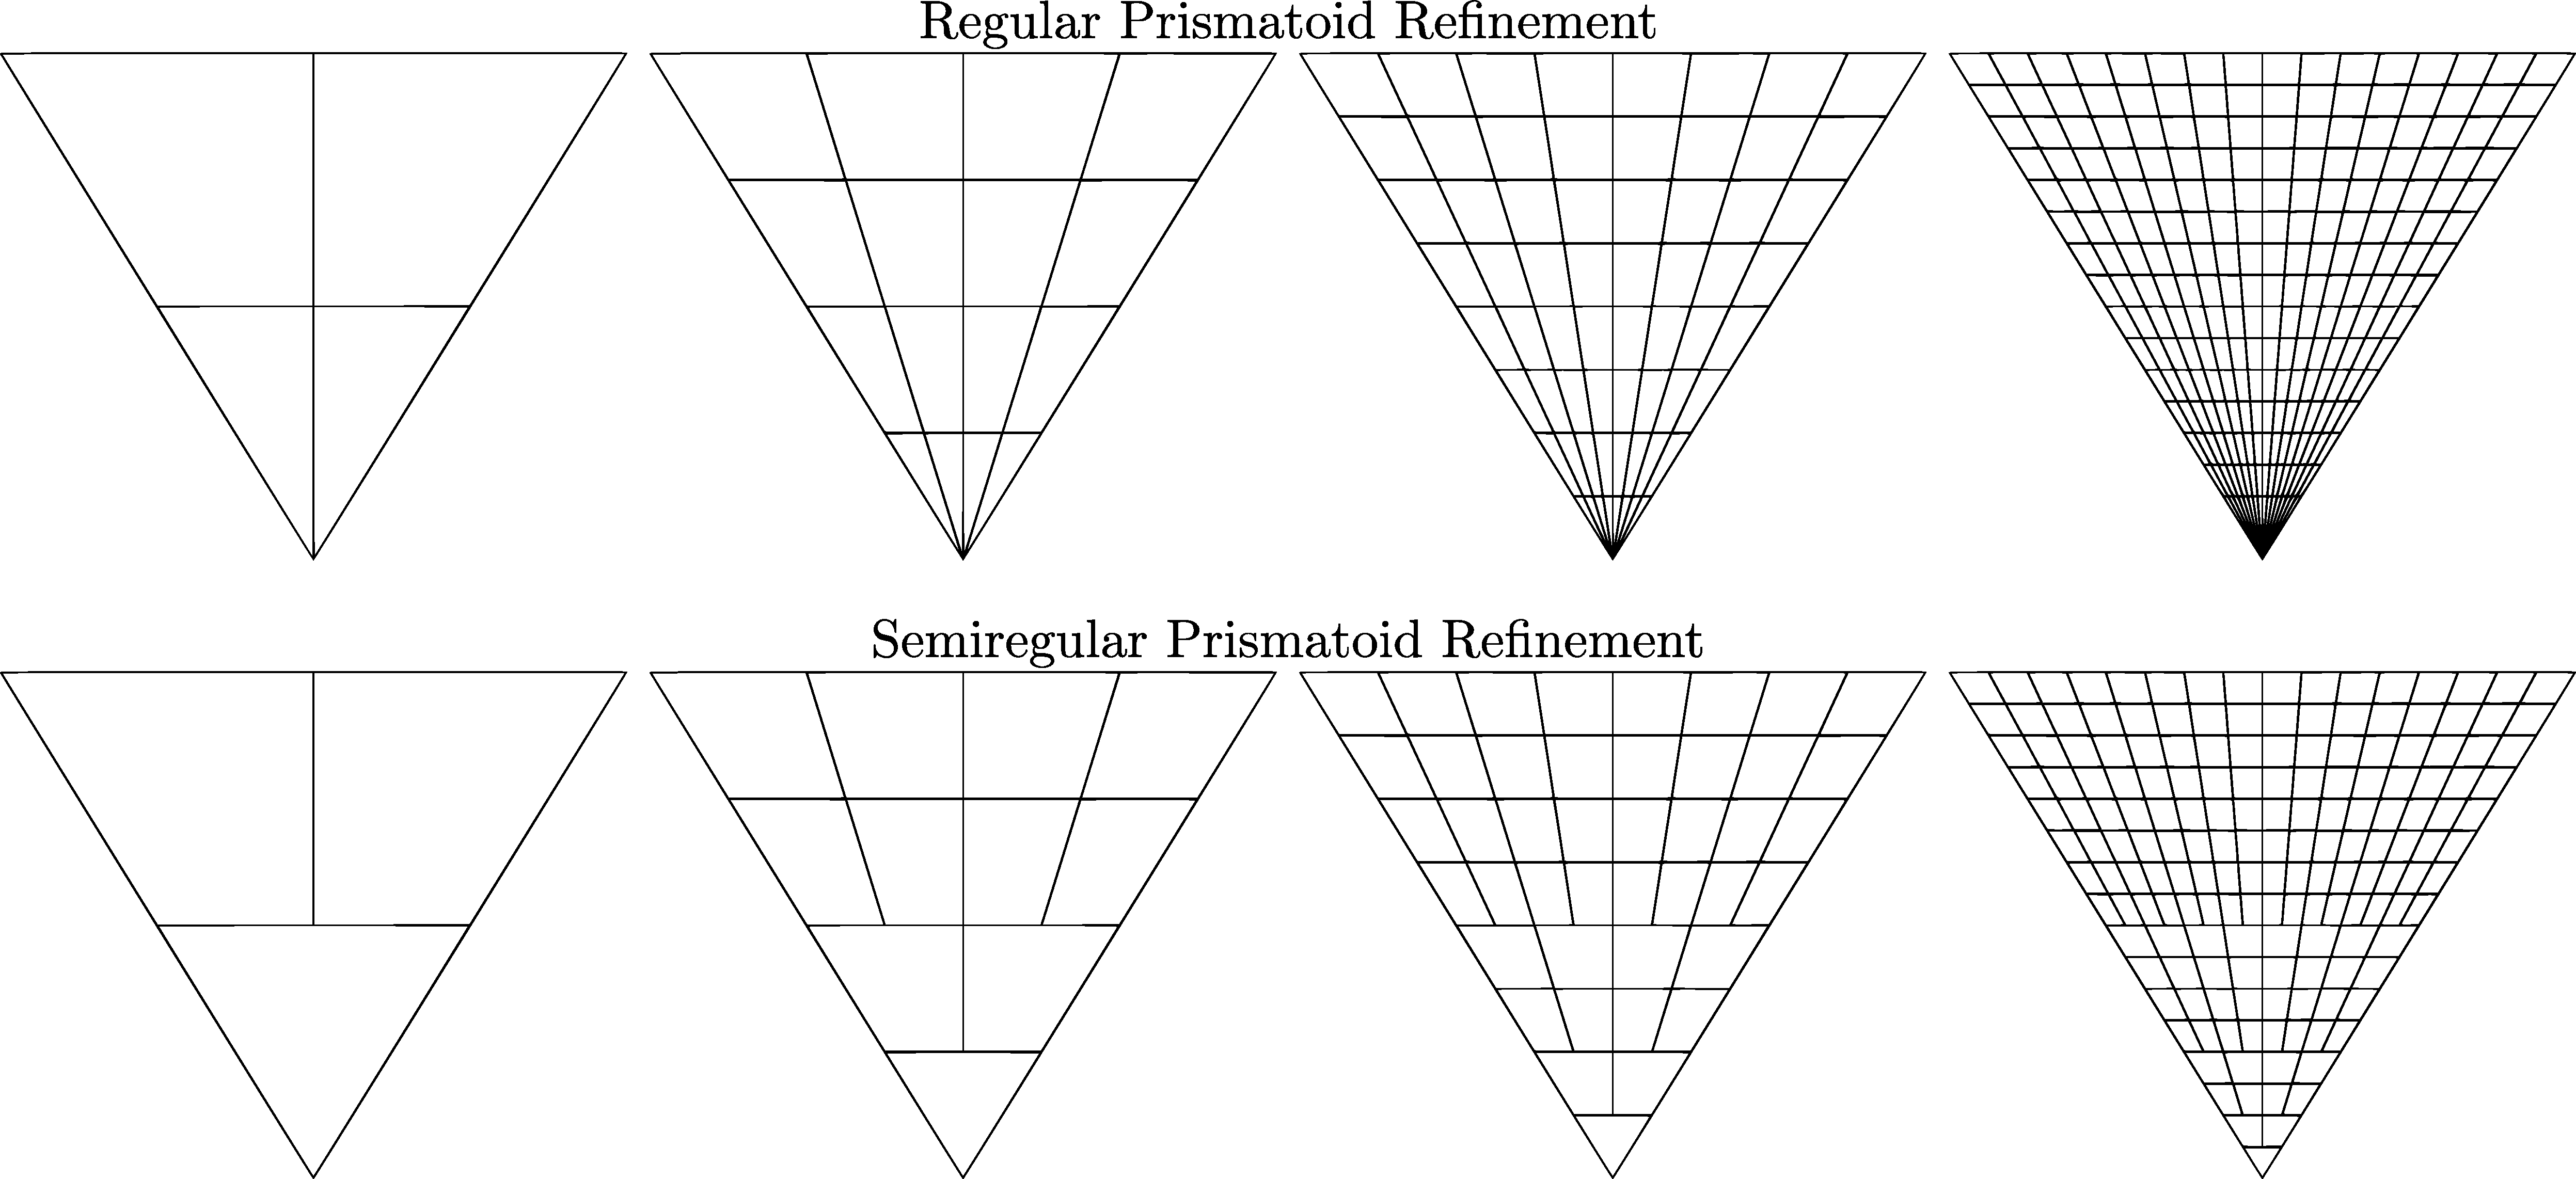
\includegraphics[width=\textwidth]{reg-vs-semireg.pdf}
	\caption[Comparison of regular and semiregular degenerate prismatoid refinement]{
		Three levels of successive applications of regular (top) and semiregular degenerate (bottom) prismatoid refinement.
		Only the side of a single pyramid starting cell is shown to highlight the behaviour of the two schemes at different radii.
		Note how cells degenerate towards the centre with regular refinement, whereas this issue is not present in the semiregular degenerate scheme
	}
	\label{fig:reg-vs-semireg}
\end{figure}


As with other semiregular degenerate refinements, normal layers in this scheme are refined using the regular method.
This regular refinement results in two normal layers, both of which have $k_s$ equal to one greater than that of the starting layer.
Figure~\ref{fig:reg-vs-semireg} compares three successive applications of regular and semiregular degenerate prismatoid refinement to a single pyramid cell.


\subsection{Other Surface Refinement Factors} \label{chap:5:factors}
While it is possible to use the above refinement methods for surface refinement factors other than 1:4, doing so results in a potentially significant issue that should be addressed.
First, we introduce the idea of a one-dimensional (1D) refinement factor, which we find by taking the square root of the surface (2D) one.
For example, the 1D refinement factor of a 1:4 surface refinement scheme (Figures~\ref{fig:regular} and \ref{fig:semiregular}) is 1:2.
While the surface refinement scheme need not be uniform across the two dimensions, the 1D refinement factor gives an idea of the \textit{average} refinement expected along each dimension.


To create uniform cells, it is clear that the refinement factor along the radial dimension for regular prismatoid refinement should be equal to the 1D refinement factor.
If this is not the case, then the width of cells relative to their depth is not constant between refinement levels, since one dimension is refined more quickly.
For a surface refinement factor of 1:4, the single radial split used matches this exactly (one split creates two new layers).
For other surface refinement factors, the 1D and radial refinement factors are not necessarily equal, and cell shape will degenerate---becoming either increasingly narrow or wide---as refinement continues.


To address this issue, we modify the number of radial splits performed such that the number of layers produced is equal to the 1D refinement factor.
For surface refinement factors that are perfect squares (e.g.
1:4, 1:9) this is trivial, as the 1D refinement factor is an integer; the corresponding radial refinement factor is achieved by creating a number of layers equal to the 1D factor.
For other surface refinement factors, though, this becomes more difficult.
The 1D refinement factor is no longer an integer, and since we can only perform a whole number of radial splits, the 1D and radial refinement factors cannot be exactly equal.
Therefore, we propose performing a different number of radial splits at different levels of refinement to make the \textit{average} radial refinement factor equal to the 1D one.


There are a few different methods that can be used to determine the number of radial splits to perform at a given refinement level.
The most straightforward method is to alternate between producing one layer (i.e.
no splits) and producing a number of layers equal to the surface refinement factor.
When the surface refinement factor is not a prime number, a better method is to alternate between the two members of a factor pair, such as two and three for a 1:6 surface factor.
In general, the product of the number of layers at each level of refinement should be equal (or as close as possible) to the 1D refinement factor to the power of the number of refinement levels.
Formally,
%
\begin{equation*}
\prod_{i = 1}^{k} \ell_{i} = f^{k},
\end{equation*}
%
where $\ell_{i}$ is the number of layers produced at refinement level $i$, $k$ is the level of refinement, and $f$ is the 1D refinement factor.
We use this equation iteratively to find the best number of layers for successive levels of refinement with prime surface refinement factors.
Table~\ref{tab:layers} lists our proposed layering sequences for surface refinement factors from 1:2 up to 1:9.


\begin{table}[ht!]
	\centering
	\caption[Layering sequences for different surface refinement factors]{
		Our proposed layering sequences for different surface refinement factors.
		Each number in the sequence is how many layers \textit{normal} layers should split into at the corresponding level of refinement.
		An overline indicates that the sequence repeats indefinitely.
		For semiregular prismatoid refinement, since the initial discretization has no normal layers, these sequences are used starting with the \textit{second} level of refinement
	}
	\begin{tabular}{@{} c l @{}}
		\toprule
		Surface Refinement Factor & Layering Sequence         \\ \midrule
		1:2                  & $\overline{2,1}$               \\
		1:3                  & $\overline{3,1}$               \\
		1:4                  & $\overline{2,2}$               \\
		1:5                  & $2,3,2,2,2,3,2,2,2,3,2,2,3...$ \\
		1:6                  & $\overline{3,2}$               \\
		1:7                  & $3,2,3,3,2,3,3,2,3,3,3,2,3...$ \\
		1:8                  & $\overline{4,2}$               \\
		1:9                  & $\overline{3,3}$               \\ \bottomrule
	\end{tabular}
	\label{tab:layers}
\end{table}


\begin{figure}[ht!]
	\centering
	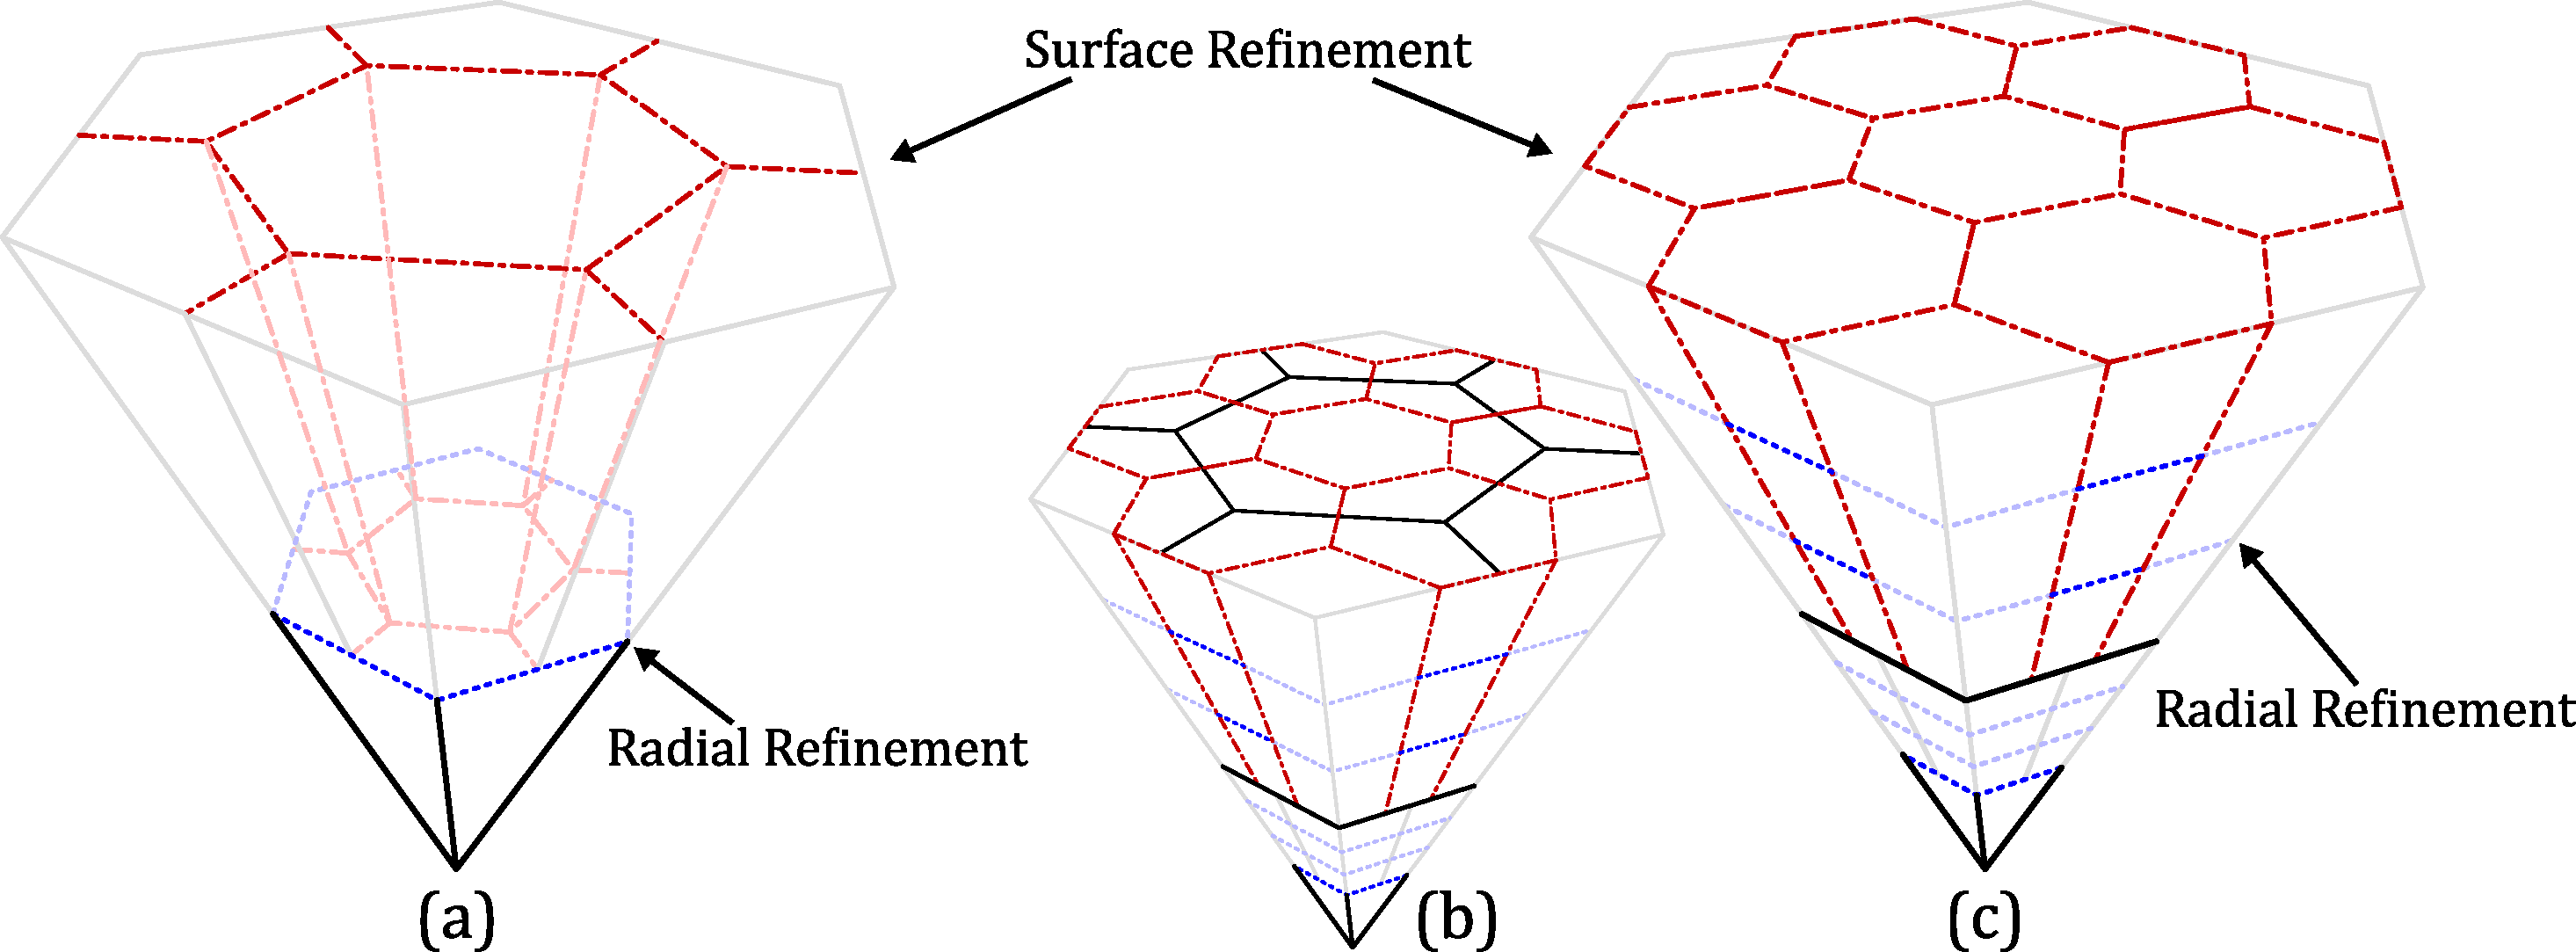
\includegraphics[width=\textwidth]{semireg-hexagons.pdf}
	\caption[Semiregular prismatoid refinement for hexagons]{
		Semiregular prismatoid refinement applied to a hexagonal base cell using a 1:3 surface refinement scheme (a) once and (c) twice; (b) is the same image as (c), but with the surface cells of the previous refinement level shown for reference.
		Note that in the second level of refinement, normal layers have two radial refinements as opposed to one
	}
	\label{fig:hexagons}
\end{figure}


Figure~\ref{fig:hexagons} showcases an example of semiregular prismatoid refinement with a 1:3 hexagonal surface refinement.
The first level of refinement is identical to the cases for a 1:4 surface refinement factor since no normal layers have been refined.
In the second level, however, two radial splits are performed in the normal layers as opposed to one.
In the next level of refinement (not shown), normal layers would not have any radial refinements per the proposed sequence in Table~\ref{tab:layers}.


\section{Cell Aspect Ratio} \label{chap:5:ar}
The surface and radial dimensions of Earth are inherently very different, and because of this, it is often desirable for these two dimensions to be at different resolutions in a 3D DGGS.
For our 3D DGGS's, achieving this entails changing the width of cells in the grid (surface resolution) relative to their depth (radial resolution).
We refer to the ratio between a cell's width and depth as the \textit{aspect ratio} of the cell.
While the refinement methods described thus far produce cells with a similar aspect ratio---both between cells in the same and different resolutions---there is no direct mechanism for controlling what this aspect ratio will be.
To address this issue, we introduce two modifications that can be made to prismatoid refinement to decrease and increase this aspect ratio.


In order to decrease the aspect ratio of cells in the grid, we must increase the number of applications of the surface refinement relative to the number of radial splits.
Since further applications of the prismatoid refinement will maintain the expected cell aspect ratio---a result of the surface and expected radial refinement factors being equal---this only needs to be done the first time a layer would have the bases of its cells refined with the surface scheme.
Thus, for semiregular prismatoid refinement, this is done while refining the outer normal layer that results from refining central layers.
%In the case where only regular prismatoid refinement is used, this is then only done during the first level of refinement.


Likewise, to increase the aspect ratio of cells, we need to decrease the number of times the surface refinement scheme is applied relative to the number of radial splits.
We accomplish this by \textit{not} applying the surface refinement to a layer the first time it would usually be done, and if needed applying additional radial splits at the same time.
These modifications would be done at the same time as the method for decreasing the aspect ratio for the same reasons.


Therefore, given some target cell aspect ratio $a$, we must determine which of the above methods to use.
To do this, we must first quantify the width and depth of a cell.
More specifically, we need to define the average width and depth of cells in a layer, since refinement is performed by layer and not by cell.
Depth comes trivially from the radial extent of the layer ($r_\mathrm{max} - r_\mathrm{min}$).
There are many potential ways to measure the width of a cell; for our purposes, we chose to use the square root of its area.
This choice ensures the framework will produce consistent results for input polyhedra with the same number of faces, irrespective of the shape(s) of said faces.


For the region of outer normal layer(s) generated by refining central layers, the average depth of cells is the total depth of the region divided by the number of layers in the region (assuming no applications of the surface refinement scheme).
Let $\upsilon$ be the percentage of $r_\mathrm{max}$ occupied by this region and $x$ be the number of extra radial splits, then the average depth of cells is
%
\begin{equation*}
\frac{\upsilon r_\mathrm{max}}{x+1}.
\end{equation*}
%
Likewise, the average cell width in this region is the surface area of the sphere divided by the number of cells (assuming no extra radial splits).
Let $n$ be the number of faces on the input polyhedron and $w$ be the number of times the surface refinement is applied, then the number of cells is $n f^{2w}$, and the average cell width is
%
\begin{equation*}
\sqrt{ \frac{ 4 \pi r_\mathrm{max}^2 }{ n f^{2 w} } } = \frac{2 r_\mathrm{max}}{f^w} \sqrt\frac{\pi}{n}.
\end{equation*}
%
We now equate these using the desired aspect ratio to solve for $x$ and $w$, giving
%
\begin{equation*}
a \frac{\upsilon}{x+1} = \frac{2}{f^w} \sqrt\frac{\pi}{n}.
\end{equation*}
%
As to not violate our prior assumptions, when solving for one variable the other is set to zero; this ensures only one of the two strategies for modifying the aspect ratio is employed.
Setting $w = 0$ we get
%
\begin{equation}
x = \frac{a \upsilon}{2} \sqrt{\frac{n}{\pi}} - 1,
\label{eq:extraSplits}
\end{equation}
%
and setting $x = 0$ we get
%
\begin{equation}
w = \log_{f} \left( \frac{2}{a \upsilon} \sqrt{ \frac{\pi}{n}} \right).
\label{eq:num2D}
\end{equation}


\begin{figure*}[ht!]
	\centering
	\begin{subfigure}[]{0.25\textwidth}
		\centering
		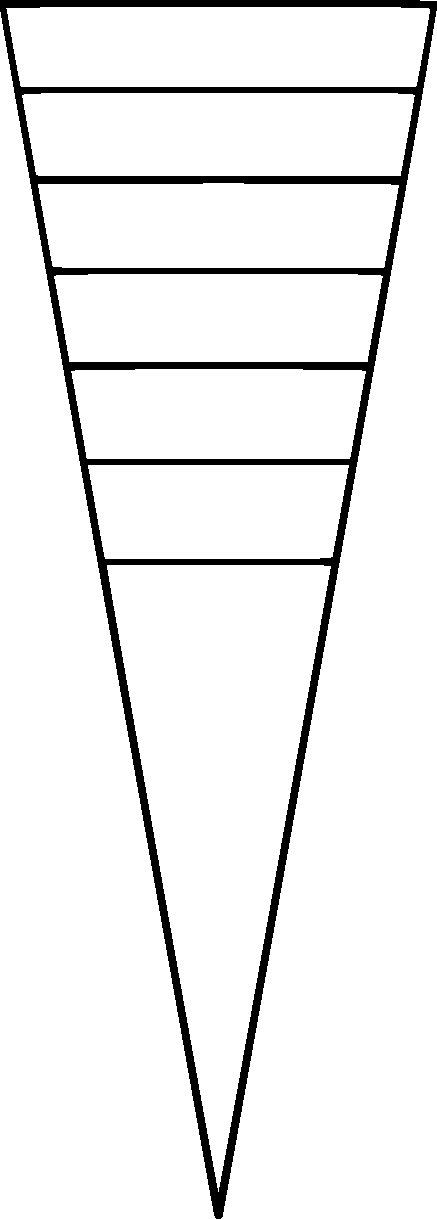
\includegraphics[width=0.5\columnwidth]{5-ers.pdf}
		\caption{}
		\label{fig:ers1}
	\end{subfigure}%
	%
	\begin{subfigure}[]{0.25\textwidth}
		\centering
		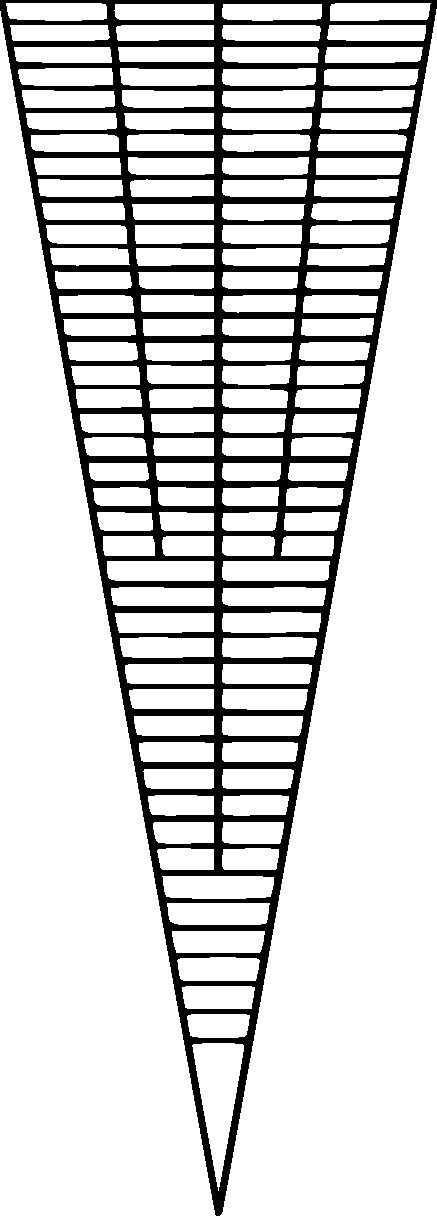
\includegraphics[width=0.5\columnwidth]{5-ers3.pdf}
		\caption{}
		\label{fig:ers3}
	\end{subfigure}%
	%
	\begin{subfigure}[]{0.25\textwidth}
		\centering
		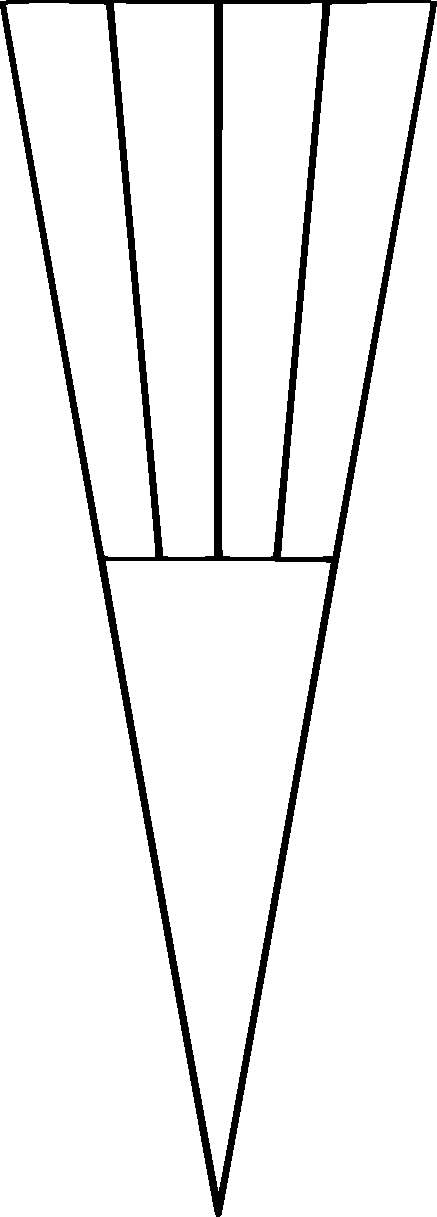
\includegraphics[width=0.5\columnwidth]{2-ess.pdf}
		\caption{}
		\label{fig:ess1}
	\end{subfigure}%
	%
	\begin{subfigure}[]{0.25\textwidth}
		\centering
		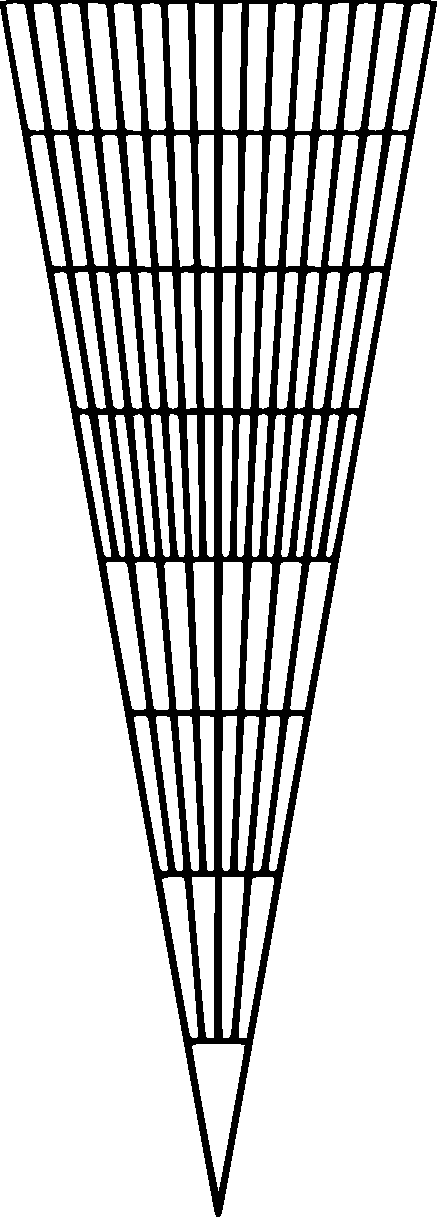
\includegraphics[width=0.5\columnwidth]{2-ess3.pdf}
		\caption{}
		\label{fig:ess3}
	\end{subfigure}
	
	\caption[Prismatoid refinement modified to achieve different cell aspect ratios]{
		A demonstration of how refinement can be modified to affect the aspect ratio of cells.
		All figures show a starting pyramid cell from a grid with 200 cells in its initial discretization.
		Central layer with five extra radial splits ($a = 3$ to get $x = 5$) at (a) one level of refinement and (b) three levels.
		Central layer with two applications of the surface refinement scheme ($a = 1/8$ to get $w = 2$) at (c) one level of refinement and (d) three levels
	}
	\label{fig:extraDPS}
\end{figure*}


The actual values of $x$ and $w$ selected for use is determined by which one is negative.
If $x$ is negative, it is set to zero, and the value of $w$ is used---vice versa for if $w$ is negative.
Since $x$ or $w$ may not be integers, we simply round them to the nearest whole number to get the actual value used during refinement.
The results of refinement with different target aspect ratios are demonstrated in Figure~\ref{fig:extraDPS}.


\section{Summary}
This chapter provides a complete and comprehensive method for extending any 2D DGGS into a 3D DGGS.
The approach is general and properly accommodates any potential DGGS regardless of the initial polyhedron, refinement, or projection employed.
Semiregular degenerate refinement allows unbounded ranges of altitudes without significant degradation in cell shape or size.
Techniques are employed to ensure cells have the desired aspect ratio while maintaining the aspect ratio and relative volume of cells during refinement.
The following chapters explain how to handle mapping and coding with these grids. 
